% \documentclass[draftcls, onecolumn, a4paper]{IEEEtran}
\documentclass[conference, a4paper]{IEEEtran}

\usepackage{amsmath}   % From the American Mathematical Society
\usepackage{amssymb}
\usepackage{amsfonts}  % A popular package that provides many helpful commands
\usepackage{graphicx}  % Required for graphics, photos, etc.
\usepackage{url}       % Written by Donald Arseneau
                        % Provides better support for handling and breaking
                        % URLs. url.sty is already installed on most LaTeX
                        % systems. The latest version can be obtained at:
                        % http://www.ctan.org/tex-archive/macros/latex/contrib/other/misc/
                        % Read the url.sty source comments for usage information.
\usepackage{cite}
\usepackage{citesort}   % nicer looking citations
\usepackage{prettyref}
\usepackage{balance}
\usepackage{subfig}   
\usepackage{xr}
\usepackage{multirow}
\usepackage{standalone}
\usepackage{pgf}
\usepackage{pgfplots}
\usepackage{verbatim}
\usepackage{tikz}
\usepackage{array}
\usepackage{booktabs}
\usepackage{xcolor}
\usetikzlibrary{arrows.meta,positioning, shapes, patterns, calc, through}
\tikzstyle{vertex}=[circle, draw, inner sep=1pt, minimum size=6pt]
\pgfplotsset{compat=1.17}
\hyphenation{}          % correct bad hyphenation here
%\DeclareAcronym{BLE}{
	short = BLE,
	long = Bluetooth-Low-Enegy
}

\DeclareAcronym{UWB}{
	short = UWB,
	long = Ultra-Wideband
}

\DeclareAcronym{TWR}{
	short = TWR,
	long = Two-Way-Ranging
}

\DeclareAcronym{EKF}{
	short = EKF,
	long = Extended Kalman Filter
}

\DeclareAcronym{IoT}{
	short = IoT,
	long = internet of things
}

\DeclareAcronym{LOS}{
	short = LoS,
	long = Line-of-Sight
}

\DeclareAcronym{NLOS}{
	short = NLoS,
	long = Non-Line-of-Sight
}

\DeclareAcronym{RTOS}{
	short = RTOS,
	long = Real-Time Operating System
}

\DeclareAcronym{TOF}{
	short = TOF,
	long = time-of-flight
}

\DeclareAcronym{TdoA}{
	short = TdoA,
	long = Time-difference-of-Arrival
}

\DeclareAcronym{PCB}{
	short = PCB,
	long = printed circuit board
}

%% acronyms and glossary
\usepackage[
single=true,
sort=true,
only-used=true
]{acro}
\DeclareAcronym{BLE}{
	short = BLE,
	long = Bluetooth-Low-Enegy
}

\DeclareAcronym{UWB}{
	short = UWB,
	long = Ultra-Wideband
}

\DeclareAcronym{TWR}{
	short = TWR,
	long = Two-Way-Ranging
}

\DeclareAcronym{EKF}{
	short = EKF,
	long = Extended Kalman Filter
}

\DeclareAcronym{IoT}{
	short = IoT,
	long = internet of things
}

\DeclareAcronym{LOS}{
	short = LoS,
	long = Line-of-Sight
}

\DeclareAcronym{NLOS}{
	short = NLoS,
	long = Non-Line-of-Sight
}

\DeclareAcronym{RTOS}{
	short = RTOS,
	long = Real-Time Operating System
}

\DeclareAcronym{TOF}{
	short = TOF,
	long = time-of-flight
}

\DeclareAcronym{TdoA}{
	short = TdoA,
	long = Time-difference-of-Arrival
}

\DeclareAcronym{PCB}{
	short = PCB,
	long = printed circuit board
}

\IEEEoverridecommandlockouts 

\begin{document}

\renewcommand{\baselinestretch}{0.97} % reduziert um auf 5 Seiten zu bleiben

\title{Ultra-Wideband (UWB) Positioning System Based on ESP32 and DWM3000 Modules}

% author names and affiliations use a multiple column layout for up to
% three different affiliations
\author{ \authorblockN{Sebastian Krebs} \authorblockN{University
    of Applied Sciences HTWG Konstanz}
  \authorblockN{Alfred-Wachtel-Str.~8, 78462 Konstanz, Germany}
  \authorblockA{Email: xxx@htwg-konstanz.de} \and
  \authorblockN{Tom Herter} \authorblockN{University
  	of Applied Sciences HTWG Konstanz}
  \authorblockN{Alfred-Wachtel-Str.~8, 78462 Konstanz, Germany}
  \authorblockA{Email: xxx@htwg-konstanz.de}
  }

% make the title area
\maketitle

\begin{abstract}
  In this paper, an \ac{UWB} positioning system is introduced, that leverages six identical custom-designed boards, each featuring an ESP32 microcontroller and a DWM3000 module from Quorvo.
  \newline
  The system is capable of achieving localization with an accuracy of up to 10\,cm utilizing \ac{TWR} measurements between one designated ''tag'' and five ''anchor'' devices.
  The gathered distance measurements are subsequently processed by an \ac{EKF} running locally on the Tag board, enabling it to determine its own position,
  relying on fixed, a priori known, positions of the Anchor boards.
  \newline
  This paper presents a comprehensive overview of the system's architecture, the key components, and the capabilities it offers for accurate indoor positioning and tracking applications.
\end{abstract}

%\vspace*{.28cm}
%\keywords{\textbf{RTLS, UWB, TOF, ESP32, DWM3000, Positioning, Tracking}}

\IEEEpeerreviewmaketitle


%%%%%%%%%%%%%%%%%%%%%%%%%
% SECTION: INTRODUCTION %
%%%%%%%%%%%%%%%%%%%%%%%%%
%%%%%%%%%%%%%%%%%%%%%%%%%
\section{Introduction}
\label{sec:Introduction}

Indoor positioning and tracking systems gain importance in a variety of industrial fields as well as in research \cite{LiFi_Positioning} \cite{Accelerometer_Positioning} \cite{UWB_Positioning} \cite{UWB_Positioning2}.

Traditional positioning systems, however, often encounter certain limitations, such as accuracy to the meter \cite{LiFi_Positioning} or an increased positioning deviation \cite{Accelerometer_Positioning}. 

In response to these challenges, Ultra-Wideband (UWB) positioning systems have emerged as a promising solution \cite{UWB_Positioning} \cite{UWB_Positioning2}.
Building on this technology, we have developed an \ac{UWB} positioning system that utilizes hardware and advanced algorithms to generate precise position information in the three-dimensional space. However, the measurements that are conducted over the course of its development are limited to the two-dimensional space only. 

The designed \ac{UWB} system consists of six identical boards that are all based on the ESP32 microcontroller, a versatile and powerful platform that is often used in low-cost \ac{IoT} scenarios \cite{ESP32}. 
These custom-made \acp{PCB} \footnote{Layout and production files are open-source available.\,\cite{uwb-tracking}} are equipped with DWM3000 modules from Quorvo, which utilizes \ac{UWB} functionalities for short-range wireless communication.

One of these boards is referred to as a ''tag''.
It is responsible for initiating measurements with the other five "anchor" boards.
The innovative aspect of the system lies in its ability to perform accurate localization without dependence on external infrastructure for its processing,
since all the necessary calculations are performed on the device itself that is being localized.

The heart of the positioning system is the \acf{EKF} implemented locally on the tag board.
This \ac{EKF} takes the distance measurements obtained by \acf{TWR} with the Anchor Boards and calculates,
and, based on their a priori known positions, calculates the real-time position of the tag board.

The system is partially scalable; the number of anchors can be significantly increased at
the expense of the general round-trip time. The ratio has the order $O(n)$.

The measuring principle of distance measurement is explained in the following section.
A distance measurement was implemented based on the associated IEEE standard  \cite{IEEE802154a} \cite{IEEE802154z}.
The chapter \ref{Section:principle} explains the system architecture,
including the choice of anchor positions and 
information about the scheduled timing in relation to position measurements.
This is followed by a brief description of the hardware designed and
its wide range of applications as a general evaluation board.
In order to explain the implementation of the firmware in more detail,
chapter \ref{section:firmware} describes the distribution of the functionalities to various tasks of the \ac{RTOS}.
The results of the static tests can be found in chapter \ref{section:tests}.
Both, the spatial resolution and the most important limitations are explained.
Finally, the last chapter summarizes the most important findings and provides a critical review of the results.



\section{Measurement Priciple}\label{Section:principle}
\acf{TWR} is a foundational technique for obtaining precise distance measurements within the UWB positioning system.
It relies on the time it takes for signals to propagate from a tag board to anchor boards and back again.
This time measurement, in compliance with the IEEE 802.15.4a/4z standards, offers the basis for distance estimation by multiplying the time traveled with the speed of light.

The following Figure \ref{fig:twr} shows how a \ac{TWR} Handshake takes place.
The Tags firmware calculates the \acf{TOF} as well as the distance between both devices by comparing the timestamps of sending and reception. 
Therefore it is necessary for the \ac{UWB} messages to not only be tracked by the time they are received at the Tag, but also to contain information about when each anchor received it and when it starts to transmit the response. 

\begin{figure}[hbt!]
	\centering
	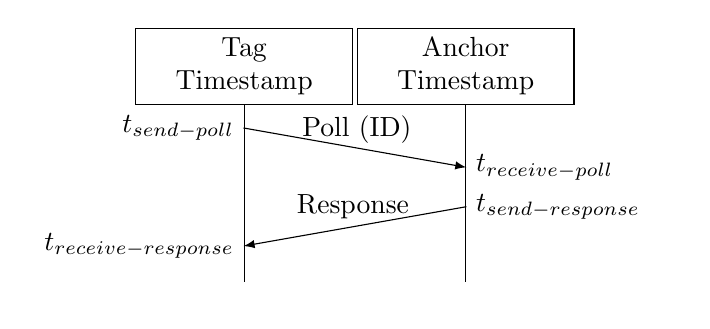
\begin{tikzpicture}[
		node distance=1.5cm,
		block/.style={
			align=center, draw,minimum width=2.75cm, minimum height=.5cm
		},
		ghost/.style={
			align=center,minimum width=0cm, minimum height=0cm
		},
		label/.style={
			minimum width=2cm, minimum height=0cm, text width=2.5cm
		},
		>=latex,
		]
		% textfields
		\node [block] (tag_timestamp) {Tag\\Timestamp};
		\node [block, right=.05cm of tag_timestamp] (anchor_timestamp) {Anchor\\Timestamp};
		
		% Endpoints
		\node [ghost, below=2.25cm of tag_timestamp] (tag_endpoint) {};
		\node [ghost, below=2.25cm of anchor_timestamp] (anchor_endpoint) {};
		
		% Timelines
		\draw [-] (tag_timestamp) -- (tag_endpoint);
		\draw [-] (anchor_timestamp) -- (anchor_endpoint);
		
		% Labels Tag-line
		\node [label, align=right, anchor=east, below=.5cm of tag_timestamp.west] (t_send_poll) {$t_{send-poll}$};
		\node [label, align=right, anchor=east, below=2cm of tag_timestamp.west] (t_receive_response) {$t_{receive-response}$};
		
		% Labels Anchor-line
		\node [label, align=left, anchor=west, below=1cm of anchor_timestamp.east] (t_receive_poll) {$t_{receive-poll}$};
		\node [label, align=left, anchor=west, below=1.5cm of anchor_timestamp.east] (t_send_response) {$t_{send-response}$};
		
		%Dotted lines
		\draw [->] (t_send_poll.east) -- (t_receive_poll.west);
		\draw [->] (t_send_response.west) -- (t_receive_response.east);
		\node [ghost, below=.5cm of anchor_timestamp.west] (poll_label) {Poll (ID)};
		\node [ghost, below=1.5cm of tag_timestamp.east] (response_label) {Response};
		
	\end{tikzpicture}
	\caption{Timing diagram of \acf{TWR}}
	\label{fig:twr}
\end{figure}

In figure \ref{fig:csvbarchart} the timing of one positioning cycle looked like during the static tests taking place in section \ref{section:tests} where five Anchor devices were utilized. 
The total time for a position estimation is set to be 250\,ms, giving each distance measurement of just 50\,ms. 
\textcolor{red}{Fühlt sich so an als würd hier noch was fehlen aber k.a. was. halt bvisschen mehr zu figure 2}

\begin{figure}
	\centering
	\begin{tikzpicture}
	\begin{axis}[
		ybar=0pt,
		bar width=10pt,
		bar shift=5pt,
		xlabel={Time [ms]},
		ylabel={Anchor index},
		ymin=0, ymax=6,
		xmin=0, xmax=500,
		legend style={at={(0.83,0.97)},
		anchor=north,legend columns=1},
		ymajorgrids=true,
		grid style=dashed,
		]
		\addplot table[col sep=comma, x=Data, y=Poll]{timing.csv};
		\addplot table[col sep=comma, x=Data, y=Response]{timing.csv};
		\legend{Poll, Response}

		% Add a dashed line at x=250
        \draw [thick=4pt] (axis cs:250,\pgfkeysvalueof{/pgfplots/ymin}) -- (axis cs:250,\pgfkeysvalueof{/pgfplots/ymax});
        \node at (axis cs:250,\pgfkeysvalueof{/pgfplots/ymin}+3) [below, rotate=90] {round-trip time};
    
	\end{axis}
	\end{tikzpicture}
	\caption{Timing diagram of the \ac{TWR} measurements.}
	\label{fig:csvbarchart}
\end{figure}

For detailed technical specifications and methods, interested readers are referred to the documentation of the IEEE 802.15.4a/4z standards \cite{IEEE802154a} \cite{IEEE802154z}, which provides comprehensive guidelines for the orchestration of \ac{UWB} signals and the calculation of \ac{TOF}.
These standards ensure the correctness and accuracy of our distance measurements.

\section{System Architecture}\label{section:system_arch}
In the presented scenario, five anchors are strategically distributed throughout the room,
positioned at a height of 4\,m just under the ceiling to maximize the likelihood of 
\ac{LOS} conditions, as it facilitates more accurate \ac{TOF} measurements, by minimizing interference caused by multipath propagation, and enhance signal reliability, leading to more precise and reliable distance calculations than in an \ac{NLOS} environment.
These five anchors do not rely on any information specific to their mounting position.

During the setup of the system the anchor positions are being transmitted to the Tag via a \ac{BLE} interface. 
The tag leverages these provided anchor positions, in conjunction with distance measurements, to determine its own position. 

The following figure \ref{fig:systemarch} illustrates the interactions between the individual components.
%It is clear that when selecting the anchor positions while setting up on a new location, that they should be evenly distributed along all three axes.
%In addition, an overhead perspective helps to reduce measurement inaccuracies.

\begin{figure}[hbt!]
	\centering
	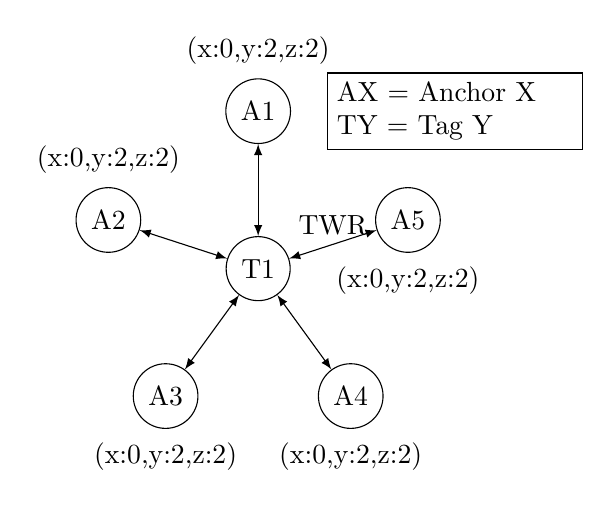
\begin{tikzpicture}[
		node distance=1.5cm,
		device/.style={
			align=center, circle, draw, minimum width=.25cm, minimum height=.5cm
		},
		ghost/.style={
			align=center,minimum width=0cm, minimum height=0cm
		},
		label/.style={
			draw, minimum width=2cm, minimum height=0cm, text width=3cm
		},
		>=latex,
		]
		% Responders with coords
		\node [device] (device2) at (90:2cm) {A1};
		\node [ghost, above=.05cm of device2.north] (dev2) {(x:0,y:2,z:2)};
		\node [device] (device3) at (162:2cm) {A2};
		\node [ghost, above=.05cm of device3.north] (dev3) {(x:0,y:2,z:2)};
		\node [device] (device4) at (234:2cm) {A3};
		\node [ghost, below=.05cm of device4.south] (dev4) {(x:0,y:2,z:2)};
		\node [device] (device5) at (306:2cm) {A4};
		\node [ghost, below=.05cm of device5.south] (dev5) {(x:0,y:2,z:2)};
		\node [device] (device6) at (18:2cm) {A5};
		\node [ghost, below=.05cm of device6.south] (dev6) {(x:0,y:2,z:2)};
		
		%Initiator
		\node [device] (device1) at (0,0) {T1};
		
		% TWRs
		\draw [<->] (device1) -- (device2); 
		\draw [<->] (device1) -- (device3); 
		\draw [<->] (device1) -- (device4); 
		\draw [<->] (device1) -- (device5); 
		\draw [<->] (device1) -- node[midway, above, align=left] {TWR} (device6);
		
		%legend
		\node [label] (legend) at (2.5,2) {AX = Anchor X \\TY = Tag Y};
		
	\end{tikzpicture}
	\caption{System architecture for positioning.}
	\label{fig:systemarch}
\end{figure}

\textcolor{red}{Figure \ref{fig:systemarch} wirkt irgendwie nicht so krass informativ. ich würds vielleicvht ganz raus lassen. hab jetzt mal nichts dazu bearbeitet aber was meinst du?}

The round trip time of the system is the product of the number of anchors and the ranging time.
The time for one distance measurement could be brought down to 50\,ms per recurrence without sacrificing accuracy, leading to a general position update interval of 250\,ms with 5 anchors. 

\textcolor{blue}{
This low ranging time of 50\,ms was achieved by implementing the firmware in a interrupt-based manner for the \ac{UWB} message recognition, and utilizing the ESPs multi-core processing capabilities.
}

Detailed information about the chances taken to optimize the round-trip time by reducing each individual ranging time
is given in section \ref{section:firmware}.


\section{Hardware Design}\label{section:hardware}
The hardware design of the \ac{UWB} communication boards draws inspiration from pre-existing DWM3000 Evaluation
boards.
However, the proprietary board development enables specialized component selection, tailored to their intended use cases.
User-friendliness was a paramount consideration during the design process,
resulting in the integration of multiple user buttons and indicating LEDs for versatile purposes like triggering the initialization of the \ac{BLE} server in order to view or change the stored anchor positions. 
Additionally, the PCB incorporates a convenient on-board LiPo battery charging and protection circuit via the USB-C interface.

Notably, our PCB design ensures a consistent layout across all boards, regardless of their specific application.
Below the antennas of both the DWM3000 and ESP32, the ground filling has been selectively omitted, to ensure antenna radiation characteristics according to the corresponding data sheets and enable more precise measurements.

\section{Firmware Architecture}\label{section:firmware}
To meet the demanding timing requirements essential for \ac{TOF} measurements and enhance network round-trip times,
the firmware is based on a \ac{RTOS}.
In particular FreeRTOS \cite{FreeRTOS_2023} offers the capability to create multiple tasks, that collaborate coherently and can be executed simultaneously on each of the two cores of the ESP32 microcontroller.

The documentation of its source code is continuously made available online with the help of Doxygen and GitHub pages.
The implementation can therefore be viewed publicly\cite{doxygen-doku}.

\textcolor{blue}{In the regular tracking mode, all devices within the system execute the \ac{TOF} task, ensuring synchronized data acquisition.
}
When a device is configured as a tag,
it additionally undertakes the execution of the \ac{EKF} task.
The \ac{EKF} task processes the distance measurements generated by the \ac{TOF} task,
culminating in a precise positional estimation.

\subsection{TOF-Task}\label{section:firmware-tof}
The \ac{TOF} task is based on the example code
provided by Quorvo for \ac{TWR} measurements.
However, we have refined the functionality by structuring it in a class-based framework.
The commonalities between the Initiator and Responder roles have been
encapsulated in a common superclass.
This design decision allows us to maintain a lean and clear software structure,
reduce redundancy and simplify maintenance.

In practice, the tag, which acts as the \ac{TWR} initiator, as part of the localization architecture iterates through a list of anchors, each of which serves as an individual \ac{TWR} responder. 
The Tag, jointly with the Anchor, generates distance measurements. 
The result is a comprehensive data set that serves as the basis for coordinate calculation. 

\subsection{EKF-Task}\label{section:firmware-ekf}
The \ac{EKF} employed in our system leverages two distinct mathematical models
to achieve precise position estimation.
For readers interested in delving deeper into the theoretical foundations of the
Kalman Filter, we recommend consulting the work of Li Qiang et al. in
"Kalman Filter and Its Application"~\cite{Kalman}.
The EKF  on the tag utilizes a prediction model based on the constant velocity and trajectory model assumption.

This model serves as a fundamental tool for estimating the next position of the tag.
For potentially more dynamic systems the use of nonlinear models
for the tag movement could improve the dynamic behavior of the Kalman Filter.

The measurement model is encapsulated in the Jacobian matrix given in Equation~\ref{eq:measurementmatrix},
enabling the transformation of measured distances into accurate position estimations. 
The measurement model finds its expression in the measurement matrix $H$, 
which effectively links the measured distances to the position estimation:

\begin{equation}
	\begin{aligned}
		\Delta x_i &= x_i - x \\
		\Delta y_i &= y_i - y \\
		\Delta z_i &= z_i - z \\
		dist_i &= \sqrt{{\Delta x_i^2 + \Delta y_i^2 + \Delta z_i^2}} \\
		H &= \begin{bmatrix}
			-\frac{{\Delta x_1}}{{dist_1}} & -\frac{{\Delta y_1}}{{dist_1}} & -\frac{{\Delta z_1}}{{dist_1}} \\
			-\frac{{\Delta x_2}}{{dist_2}} & -\frac{{\Delta y_2}}{{dist_2}} & -\frac{{\Delta z_2}}{{dist_2}} \\
			\vdots & \vdots & \vdots \\
			-\frac{{\Delta x_{\text{max}}}}{{dist_{\text{max}}}} & -\frac{{\Delta y_{\text{max}}}}{{dist_{\text{max}}}} & -\frac{{\Delta z_{\text{max}}}}{{dist_{\text{max}}}}
		\end{bmatrix}
	\end{aligned}
	\label{eq:measurementmatrix}
\end{equation}
By using the matrix $H$, the \ac{EKF} is able to directly translate the position estimate into predicted distance measurements.
These are further compared to real distance measurements and based on this information the position estimate is improved.


\section{Test Results}\label{section:tests}
The implementation of localization systems often requires the evaluation of the measured values through empirical,
static and dynamic tests.
Since the dynamics of position determination are largely determined by the parameterization of the \ac{EKF},
a detailed evaluation of the system's ability to detect moving objects is not examined here.

The effect of the anchor arrangement is crucial to the success of the system.
In the case of these tests, the anchors were mounted at a height of 4m.
One single anchor was mounted at a height of 1m to ensure good position resolution in the Z axis.
Otherwise, an overestimation of the distances and, thus, a poor calculation of the Z axis was determined.

During testing, attention was paid to keep \ac{LOS} conditions with all anchors,
although tests showed that the influence of \ac{NLOS} conditions can be partially compensated for by the \ac{EKF}.
The table \ref{table:measurements} shows fixed positions in the room that were measured using the system
over a fixed period of time in a grid-like pattern. 
To do this, the mean deviation and the fluctuation of the values over the standard deviation are then evaluated. 
Before each test sequence it is ensured, that the \ac{EKF} is not biased by values of previous measurements. 

\begin{table}[hbt!]
	\centering
	\begin{tabular}{l l l c}
		%\toprule
		\textbf{Position[m]} & \textbf{$\mu$[cm]} & \textbf{$\sigma$[cm]}\\
		$(x,y)$ & $mean(length)$ & $std(length)$\\
		%\midrule
		$(2,2)$ & $67.66\,cm$ & $2.90\,cm$\\
		$(2,3)$ & $55.42\,cm$ & $2.97\,cm$\\
		$(2,4)$ & $65.05\,cm$ & $2.8\,cm$\\
		$(2,5)$ & $47.31\,cm$ & $3.51\,cm$\\
		$(2,6)$ & $46.07\,cm$ & $3.13\,cm$\\
		$(2,7)$ & $54.00\,cm$ & $3.17\,cm$\\
		$(2,8)$ & $34.48\,cm$ & $3.3\,cm$\\
		
		$(3,2)$ & $31.74\,cm$ & $3.42\,cm$\\
		$(3,3)$ & $121.37\,cm$ & $4.47\,cm$\\
		$(3,4)$ & $23.06\,cm$ & $3.07\,cm$\\
		$(3,5)$ & $29.34\,cm$ & $2.91\,cm$\\
		$(3,6)$ & $28.31\,cm$ & $2.93\,cm$\\
		$(3,7)$ & $22.68\,cm$ & $3.2\,cm$\\
		$(3,8)$ & $32.98\,cm$ & $3.73\,cm$\\
		
		$(4,2)$ & $19.75\,cm$ & $2.97\,cm$\\
		$(4,3)$ & $21.73\,cm$ & $3.4\,cm$\\
		$(4,4)$ & $29.91\,cm$ & $2.9\,cm$\\
		$(4,5)$ & $9.27\,cm$ & $3.2\,cm$\\
		$(4,6)$ & $28.1\,cm$ & $2.84\,cm$\\
		$(4,7)$ & $35.95\,cm$ & $8.34\,cm$\\
		$(4,8)$ & $14.88\,cm$ & $3.13\,cm$\\
		
		$(5,2)$ & $80.12\,cm$ & $3.61\,cm$\\
		$(5,3)$ & $61.88\,cm$ & $4.19\,cm$\\
		$(5,4)$ & $47.44\,cm$ & $3.57\,cm$\\
		$(5,5)$ & $21.28\,cm$ & $6.76\,cm$\\
		$(5,6)$ & $31.89\,cm$ & $3.65\,cm$\\
		$(5,7)$ & $33.02\,cm$ & $3.72\,cm$\\
		$(5,8)$ & $26.27\,cm$ & $3.73\,cm$\\
		
		$(6,2)$ & $89.12\,cm$ & $2.99\,cm$\\
		$(6,3)$ & $99.28\,cm$ & $4.28\,cm$\\
		$(6,4)$ & $73.01\,cm$ & $3.88\,cm$\\
		$(6,5)$ & $55.42\,cm$ & $6.16\,cm$\\
		$(6,6)$ & $10.63\,cm$ & $4.56\,cm$\\
		$(6,7)$ & $29.46\,cm$ & $7.01\,cm$\\
		$(6,8)$ & $13.0\,cm$ & $2.86\,cm$\\
		
		%\bottomrule
	\end{tabular}
	\caption{Static mesurement deviation out of 500 measurements at each grid intersection point.}
	\label{table:measurements}
\end{table}

The 10\,m\,x\,8\,m room was divided into 1\,m\,x\,1\,m squares. 
Multiple measurement was then carried out over the course of three minutes at each grid intersection point.
This procedure allows the deviations of the positions to be represented in relation to the location in the room.
For the illustration in figure \ref{fig:statistics}, $3\sigma$-ellipses were drawn to show the scattering per position.

\begin{figure}[hbt!]
	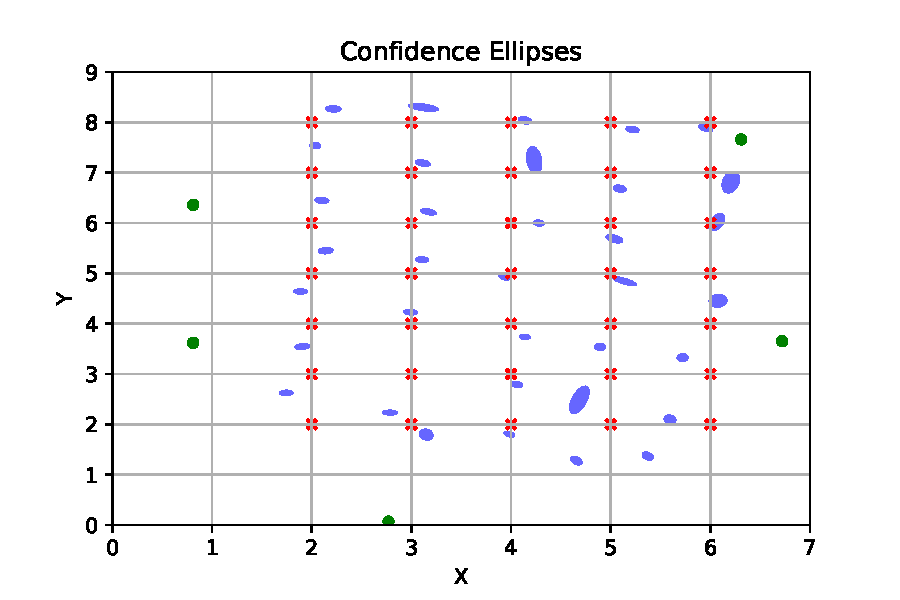
\includegraphics[scale=0.63]{pic/position_plot.pdf}
	\caption{Confidence ellipses of the grid measurement with 99.7\,\% of the points inside of the ellipse.}
	\label{fig:statistics}
\end{figure}

\textcolor{blue}{
The graph in figure \ref{fig:statistics} shows, that the biggest part of the scattering occurs in the x-direction. 
A systematic error seems to appear when taking a look at the deviation in the y direction over the x axis. 
The more distance is between the measured intersection point and the center of 4\,m\,x\,4\,m the bigger the deviation of the mean is to the actual positions. 
Furthermore positions more to the right of the center in x direction tend to have a displacement in the positive y direction, while points more to the right of the center in x direction tend toi have a negative y displacement. 
The bigger the distance is the greater this displacement gets. 
Overall the best performance is achieved in the direct center of the grid where the distance to every anchor is roughly equal.
}

%Even if the system is clearly capable of very precise positioning, it can be said that if uniform positioning accuracy is to be achieved, the best arrangement of the anchors must be determined using simulation means.
%This ensures that the propabillity of occuring "blind spots" is reduced.

\section{Conclusion And Outlook}\label{section:conclusion}
In conclusion, it can be said that a relatively precise localization system has been designed.
Both the hardware and the software were designed specifically for use as a positioning module and fulfill this purpose with a satisfying accuracy of XXX (noch einfügen und ggf. erläutern wo besser wo schlechter).

A critical point is that the system's is scalability has a linear impact on its temporal performance.
By pinging every single anchor, the tag is not able to handle a very large number of anchors without increasing the roundtrip time.
This problem could be avoided by instead of \ac{TWR} measurements \ac{TdoA} measurements would be performed.
Even if this measurement principle requires a nanosecond precise synchronization of the anchors,
the roundtrip time would be limited to the duration of one ping process.

Initially, a hybrid solution using \ac{TWR} and \ac{TdoA} measurements was planned,
but the wireless clock synchronization of the anchors is currently only possible with limited accuracy.
Further research in this area could allow the system to generate accurate position measurements with a period duration of up to 50ms.

%To achieve further improvements, we are committed to fostering collaboration and knowledge-sharing within the community.
%Therefore, we have made the entire source code, along with all PCB design files, readily accessible to the public.
%You can find these resources, along with detailed documentation, on our project's GitHub repository \cite{uwb-tracking}.



\bibliographystyle{IEEEtran} \bibliography{boid}


\end{document}

%%% Local Variables: 
%%% mode: latex
%%% TeX-master: t
%%% End: 
